\documentclass[output=paper]{langsci/langscibook}
\ChapterDOI{10.5281/zenodo.13347664}
\author{Veton Matoshi\affiliation{LMU Munich}}
\title[Clitic doubling in Albanian dialects]{Clitic doubling in Albanian dialects from the perspective of functional transparency}
\abstract{The relevant literature reports differences in the use of clitic doubling in Albanian dialects. Quantitative corpus studies show that all dialects spoken outside of the Republic of Albania show a more frequent use of clitic doubling. The data of this corpus prove that the less restrictive use of clitic doubling is not accompanied by increasing transparency of its usage. In contrast to Standard Albanian, where the usage of clitic doubling is not optional and can almost without exception be explained by topic and focus marking, in the peripheral Albanian dialects outside of the Republic of Albania numerous exceptions from the general tendency can be detected. In order to explain these exceptions, a wide variety of factors must be taken into account and, in certain contexts, point to the optional use of clitic doubling. From a descriptive point of view, these exceptions suggest an increasing degree of functional opaqueness.}

\begin{document}
\maketitle

\section{Introduction}\label{sec:matoshi:1}

Most studies on differential object marking and clitic doubling, including this one, follow a simple key question: What are the properties of objects that trigger clitic doubling? In order to approach this question from a broader perspective, it is useful to outline general aspects of typologically grounded theories on agreement and transitivity. Typological studies question the purely syntactic notion of transitivity which posits the existence of an object as a sufficient indicator of transitivity. This dichotomous view (intransitive vs. transitive) can be supplemented by a semantic approach to transitivity, which states that clauses exhibit a certain degree of transitivity depending on the pragmatic and semantic properties of the agent and the patient. The degree of transitivity can be measured on the basis of certain properties of the core arguments and the semantics of the verb. \tabref{tab:matoshi:1} summarizes the basic idea of prototypical transitivity according to \citet{Hopper1980}.

\begin{table}
\begin{tabular}{lll}
\lsptoprule
                     & \multicolumn{2}{c}{Degree of transitivity} \\
\cmidrule(lr){2-3}
Factor               & \multicolumn{1}{c}{High} & \multicolumn{1}{c}{Low}\\
\midrule
a. Participants      & 2 or more participants, A and O & 1 participant\\
b. Kinesis           & action & non-action\\
c. Aspect            & telic & atelic\\
d. Punctuality       & punctual & non-punctual\\
e. Volitionality     & volitional & non-volitional\\
f. Affirmation       & affirmative & negative\\
g. Mode              & realis & irrealis\\
h. Agency            & A high in potency & A low in potency\\
i. Affectedness of O & O totally affected & O not affected\\
j. Individuation of O & O highly individuated & O non-individuated\\
\lspbottomrule
\end{tabular}
\caption{Parameters of transitivity according to \citet[252]{Hopper1980}.\label{tab:matoshi:1}}
\end{table}

Prototypical transitive clauses exhibit an object which shows a high degree of individuation and affectedness due to the action executed by the agent which is prototypically a deliberately acting agent. For instance, definite and highly referential objects (criterion J) are analyzed as being a more typical component of transitive clauses than indefinite and less referential objects. \citet[259]{Hopper1980} go so far as to posit – more like an \enquote{extreme restatement} –  that \enquote{an indefinite O is not really an O at all, but is a subordinate part of a compound of which the verb stem is the head (i.e., it is incorporated into the verb)}.

Instances of \enquote{special} object marking can be considered, in a broad sense, as morphosyntactic realizations of a higher or lower degree of transitivity, among them:
\begin{itemize}
	\item	clitic doubling = high transitivity
	\item	differential object marking = high transitivity
	\item	object omission (anti-causative, incorporation) = low transitivity 
\end{itemize}

\noindent
Another way of viewing transitivity is the notion of distinctness of participants or the \enquote{maximally distinguished argument hypothesis} \citep{Ness2007} which states, in simple terms, that the two main participants (subject and object) must be semantically maximally distinguishable from each other. \citet[52]{Lenz1920} was one of the first to assume a distinguishing function of differential object marking. He assumed that in \ili{Spanish} the direct object bears the preposition \textit{a} only if it is logically possible to perceive it as the subject of the clause.  

The introduction so far has shown that clitic doubling can be viewed in the wider context of argument alignment and, what is more important, as a realization of differential object marking \citep{Kallulli2016}. \citet[151]{Bossong1991} regarded the emergence of differential object marking as a form of \enquote{grammemic replacement} of eroded case systems with the important difference that case systems, such as the \ili{Latin} case system, are \enquote{a petrified grammatical category whereas the more recent DOM [differential object marking] systems are living ones}. As a consequence, the former \enquote{are used mechanically and without exception} and are \enquote{meaningless}, whereas the usage of differential object marking is not pervasive and is dependent on different factors, mostly regarding the defining properties of the object and the action denoted by the verb. 

One major factor which can be associated with the emergence of a new case or agreement system is topicality. \citet[152]{Givon1976} introduces a universal hierarchy of topicality that ranks the core arguments regarding their likelihood to be topics as follows: agent $>$ dative $>$ accusative. This hierarchy serves as a starting point for Givón’s theory on the emergence of object (and subject) agreement which basically states that an overuse of the topic-shift construction will eventually lead to the grammaticalization of object agreement, including clitic doubling in this context, cf. \tabref{tab:matoshi:2}.

\begin{table}
\begin{tabular}{L{.25\textwidth}L{.3\textwidth}L{.25\textwidth}}
\lsptoprule
topic shift (\enquote{marked}) & afterthought-topic construction (\enquote{semi-marked}) & neutral (\enquote{demarked})\\
\midrule
\textit{The man, I saw him.} & \textit{I saw him, the man.} & \textit{I saw-him, the man.}\\
\lspbottomrule
\end{tabular}
\caption{Grammaticalization of object agreement via topic-shift constructions according to \citet[157]{Givon1976}.\label{tab:matoshi:2}}
\end{table}

Very often topic and focus are viewed as being in a complementary distribution (see for example \citealt[538]{Buchholz1987}, \citealt[218]{Kallulli2000} for \ili{Albanian}), which is reminiscent of what is traditionally called topic and comment. It should not go unmentioned that major caveats have been expressed concerning such a definition of topic and focus (see for example \citealt[30]{Leafgren2002}). The absence of a widely accepted definition of the terms \textit{topic} and \textit{focus} and their importance for clitic doubling in \ili{Albanian} require a general definition of the terms as they are used in this article. The term \textit{topic} is used according to the notion of \textit{aboutness}-topic, thus the \enquote{topic of a sentence is the thing which the proposition expressed by the sentence is about} \citep[118]{Lambrecht1994}. Focus, on the other hand, \enquote{refers to significant emphasis on a particular element within the context of the information conveyed in a particular clause} \citep[23--24]{Leafgren2002}. It becomes clear that these definitions call into question the view of a complementary distribution of topic and focus. They do not, however, refute the view that in the majority of cases topic and focus do not overlap, as it is usually the part of a clause which conveys the new information that also bears a significant emphasis and consequently stands out. This gradual tendency can be depicted using a modified version of the topic acceptability scale of \citet[165]{Lambrecht1994} in \tabref{tab:matoshi:3}.\largerpage[-1]

\begin{table}[h]
\begin{tabular}{ll>{\columncolor{lightgray}}l}
\lsptoprule
active                  & most acceptable topic &least acceptable focus\\
accessible              & \multicolumn{1}{c}{\multirow{3}{*}{\huge$\downarrow$}} & \\
unused                  & & \\
brand-new anchored      & & \multicolumn{1}{c}{\multirow{-3}{*}{\cellcolor{lightgray}\huge$\uparrow$}}\\
brand-new unanchored    & least acceptable topic & most acceptable focus\\         
\lspbottomrule
\end{tabular}
\caption{Topic acceptability scale according to \citet[165]{Lambrecht1994} (the grey part is a modification by the author).\label{tab:matoshi:3}}
\end{table}

The theoretical framework outlined above allows the general statement that objects which incorporate the typical properties of a subject, such as [+animate\slash human, +definite, +specific, +given, +topic, \textminus{}focus] are prone to some sort of differential marking. This is, simply put, the basic idea behind the theory of grammaticalization of differential object marking along the referentiality hierarchy, cf. \figref{fig4}.

\begin{figure}[ht]
\includegraphics[width=\textwidth]{figures/matoshi1.png}
% % \begin{forest} for tree = {fit=tight}
% % [Human pronoun
% %   [Human PN
% %       [Human definite
% %           [Human specific
% %               [Human non-specific
% %                   [,phantom]
% %                   [Animate non-specific
% %                       [,phantom]
% %                       [Inanimate non-specific]
% %                   ]
% %               ]
% %               [Animate specific]
% %               ]
% %           [Animate definite]
% %       ]
% %       [Animate PN]
% %   ]
% %   [Animate pronoun
% %       [Inanimate pronoun
% %           [Inanimate PN
% %               [Inanimate definite
% %                   [Inanimate specific]
% %                   [,phantom]
% %               ]
% %               [,phantom]
% %           ]
% %           [,phantom]
% %       ]
% %   ]
% % ]
% % \end{forest}
\caption{\label{fig4}Grammaticalization of differential object marking along the referentiality hierarchy \citep[459]{Aissen2003}.}
\end{figure}
 
The theory implies that at the end of the grammaticalization process all objects, irrespective of their pragmatic-semantic quality, will undergo clitic doubling or, as \citet[152]{Bossong1991} puts it, \enquote{such a differential system may ultimately become non-differential again}.\largerpage[-1]

An intuitive conclusion would be to associate an increasing grammaticalization of differential object marking with a loss of restrictive usage rules, more freedom of use and consequently, in the broadest sense, a language change for the better. Note, however, that \figref{fig4} viewed in isolation, suggests well-defined intermediate stages, which does not do justice to the fact that grammaticalization is a continuous process with several transitional stages which, in turn, may allow a certain extent of optionality. Optional differential object marking is evidenced for many languages, such as \ili{Sinhalese}, \ili{Romanian}, and \ili{Yiddish} \citep{Aissen2003}. Such cases cannot be explained on the basis of well-defined factors or rules and can be considered, at least from a descriptive point view, as functionally less motivated and therefore opaque. The leading question will be: Does a higher degree of grammaticalization and, therefore, a less restricted usage of clitic doubling consequently lead to a higher degree of functional transparency? Or does an increased frequency of usage lead to the disappearance of a stable system and therefore result in a higher degree of optionality and functional opaqueness in certain contexts? This question will be pursued on the basis of a quantitative and qualitative corpus analysis of clitic doubling in \ili{Albanian} dialects.

\section{Clitic doubling in Albanian}

\subsection{Syntax of clitic doubling in Albanian}

\ili{Albanian}, as a member of the so-called \textit{Balkan Sprachbund}, shares some structural similarities with surrounding languages which cannot be attributed to genealogical relationships, but rather to intensive language contact. It is important to note that these similarities go beyond lexical borrowings or phonological approximations and extend to the level of morphosyntax \citep{Friedman2006}, one case being clitic doubling. In the case of \ili{Albanian} and other Balkan languages, clitic doubling constitutes an additional marking of the direct or indirect object with depronominal clitics; cf. \REF{example1matoshi}, where the clitic \textit{e} is coreferential to \textit{djalin} ‘the boy’. Note: In the translations the accusative clitic in the 3rd person is always indicated by a \textsc{cl} and its absence with a $\varnothing$.
 \ea \label{example1matoshi} 
 	\langinfo{Northwest Gheg}{Montenegro}{42.43041, 19.25936}\footnote{Most language examples have glosses. If an example exceeds a certain length, only the translation is given. The information given for each example are: \ili{Albanian} dialect, country, geographical coordinates (longitude and latitude). If not otherwise stated, all examples are taken from a dialect corpus which was compiled for this study that is described in \sectref{sec:matoshi:3.1}. \sectref{sec:matoshi:3.1} gives an overview of modern \ili{Albanian} dialects.}\\
 	\gll {Plaka} {\uline{e}} {ndali} {\uline{djalin}} {me} {têtjë} {me} {tê} \\
 	old\_woman.\textsc{nom.def} \textsc{cl.acc.3sg} \textsc{stop\textsc{.aor.3sg}} boy.\textsc{acc.def} \textsc{inf} stay.\textsc{ptcp} with her \\
    \glt ‘The old woman \textsc{cl} stopped the boy so that he would stay with her.\il{Northwest Gheg}’
 \z

In contrast to other Balkan languages, the inventory of pronominal clitics in \ili{Albanian} is rather simple since they show no gender distinction and dative and accusative clitics in the 1st and 2nd person coincide in their form, cf. \tabref{tab:matoshi:4}.


\begin{table}
\caption{\label{tab:matoshi:4}Paradigm of pronominal clitics in Standard Albanian. Some dialects may show slightly different paradigms.}

\begin{tabular}{>{\scshape}lcc}
\lsptoprule
 & Dative & Accusative \\
\midrule
\oldstylenums{1}sg & \multicolumn{2}{c}{\textit{më}}        \\
\oldstylenums{1}pl & \multicolumn{2}{c}{\textit{na}}        \\
\oldstylenums{2}sg & \multicolumn{2}{c}{\textit{të}}        \\
\oldstylenums{2}pl & \multicolumn{2}{c}{\textit{ju}}        \\
\oldstylenums{3}sg & \textit{i}  & \textit{e}     \\
\oldstylenums{3}pl & \textit{u}  & \textit{i}     \\
\lspbottomrule
\end{tabular}
\end{table}

Clitics appear mostly as proclitics, i.e. preceding either the inflected verb, compare (\ref{example1matoshi}), or the main verb in an infinite verbal construction, compare (\ref{example2matoshi}).

\ea
 \label{example2matoshi} 
	\langinfo{Northeast Gheg}{Serbia}{42.30917, 21.64986}\\
	\gll Ridvani don me \uline{ja} falë \uline{lojën} edhe e hup \\
	Ridvan.\textsc{nom.def} want.\textsc{prs.3sg} \textsc{inf} \textsc{cl.dat.3sg.cl.acc.3sg} give.\textsc{ptcp} game.\textsc{acc.def} and \textsc{cl.acc.3sg} lose.prs.3sg \\
	\glt ‘Ridvan wants to let him win and loses the game.’ (Lit. ‘Ridvan wants to \textsc{cl} give him \uline{the game} and loses it.’\il{Northeast Gheg})
\z

Clitics can be attached to the verb stem in combination with imperative verb forms, cf. (\ref{example3matoshi}).

\ea \label{example3matoshi}
	\langinfo{Northwest Gheg}{Montenegro}{42.43041, 19.25936}\\
	\gll Hê, ktu tek jam, po çil-\uline{ma}-ni \uline{derën} \\ 
	\textsc{interj} here at be.\textsc{prs.1sg} so open-\textsc{cl.dat.1sg.cl.acc.3sg-prs.2pl} door.\textsc{acc.def} \\
	\glt ‘Hey, here I am, so open-\textsc{cl} \uline{the door} for me.\il{Northwest Gheg}’
\z

\subsection{Use of clitic doubling}\label{sec:matoshi:2.2}

One major function of the clitics is the phoric resumption of discourse referents; cf. (\ref{example4matoshi}), where the \textit{të shoqen dhe të dy ushtarët} ‘his wife and both soldiers’ are referenced in the subsequent sentence with a clitic. This usage of pronominal clitics will not be addressed in this paper.

\ea \label{example4matoshi} 
	\langinfo{South Gheg}{Albania}{41.90111, 20.0475} \\
	\gll Sa vajtën, mreti \uline{e} njofti \uline{të} \uline{shoqen} \uline{dhe} \uline{të} \uline{dy} \uline{ushtarët}. \uline{I} pyti se si ish puna \\ once go.\textsc{aor.3pl} king.\textsc{nom.def} \textsc{cl.acc.3sg} recognize.\textsc{aor.3sg} \textsc{art} wife.\textsc{acc.def} and \textsc{art} two soldier.\textsc{acc.pl.def} \textsc{cl.acc.3pl} ask\textsc{.aor.3sg} that how be.\textsc{ipf.3sg} matter.\textsc{nom.def} \\
	\glt ‘The moment they came, the king \textsc{\uline{cl}} recognized \uline{his wife and both soldiers}. He \textsc{cl}(=them) asked what their story was.\il{South Gheg}’
 \z

Without exaggeration it can be said that almost any research on clitic doubling in \ili{Albanian} focuses on 3rd person accusative clitic doubling. This interest in 3rd person accusative clitic doubling is due to the simple fact that all dative objects and 1st/2nd person accusative objects are unexceptionally doubled \citep[444]{Buchholz1987}. On the other hand, grammarians have struggled to determine the usage of 3rd person accusative clitic doubling (hereafter clitic doubling if not stated otherwise) with a great amount of certainty \citep[3--4]{Buchholz1977}.

Clitic doubling can only occur if the associated nominal or pronominal phrase has the syntactic status of direct object. Nominal phrases in the accusative which do not qualify as such cannot be associated with a coreferential clitic. Thus, bare nominal indefinites are never doubled \citep{Kallulli2016}. These cases can typically be found in recurrent light verb constructions, cf. (\ref{example5matoshi}), but less frequent constructions fall under this category also, cf. (\ref{example6matoshi}).    
\ea \label{example5matoshi} 
	\langinfo{South Tosk}{Albania}{40.2115, 19.68922}\\
	\gll Finoku as hante sa duhej, as \uline{bënte} \uline{muhabet} si përpara \\
	Finok.\textsc{nom.def} neither eat.\textsc{ipf.3sg} as\_much\_as need.\textsc{ipf.pass.3sg} neither do.\textsc{ipf.3sg} conversation as before \\
	\glt ‘Neither did Finoku eat as much as he should, nor did he $\varnothing$ \uline{have conversations} like before.’\il{South Tosk}
\ex \label{example6matoshi} 
	\langinfo{North Tosk}{Albania}{40.52797, 20.97003}\\
	\gll Plaka \uline{gjen} \uline{ustallarë} dhe fillojnë ndërtimin\\
	old\_woman\textsc{.nom.def} find.\textsc{prs.3sg} mason.\textsc{pl} and begin.\textsc{prs.3pl} constructing.\textsc{acc.def}\\
	\glt ‘The old woman $\varnothing$ finds masons and they start to build.’\il{North Tosk}
 \z
According to the notion of transitivity, as outlined in \sectref{sec:matoshi:1}, the status of the noun phrases in (\ref{example5matoshi}) and (\ref{example6matoshi}) as object becomes questionable in favor of another analysis, namely considering them as components of a verbal incorporation.\largerpage[2]

Once the status as a genuine direct object is identified, the use of clitic doubling becomes contingent on information structure. \citet[192]{Buchholz1977} and later \citet[440]{Buchholz1987} cite the \enquote{primary accent} (\textit{Primärakzent}), i.e. focus, as an important factor, stating that clitic doubling is applied if the object is topicalized\footnote{They use the terms \textit{theme} and \textit{rheme}.} and not within the focus domain, which, in general, is in compliance with the descriptions we find in other standard grammars \citep{Agalliu2002} and in recent works on clitic doubling in \ili{Albanian} \citep{Kallulli2016}. This systematicity is well depicted in (\ref{example7matoshi}): when the key to room forty is mentioned for the first time in an object position, it is not doubled. In the subsequent clause, when the same referent, the key to room forty, occurs again in the object position and is topicalized, it undergoes clitic doubling.

\ea \label{example7matoshi} 
	\langinfo{North Tosk}{Albania}{40.52797, 20.97003}\\
	\textit{Ky djali, pas një kohe, si u rrit, i kërkon të jëmës çelsat e pallatit. Dhe ajo i thotë se: - Çfarë të duhen ty çelsat?- Unë i dua, të di se çfarë ka në pallat. E ëma i jep tridhjetë e nëndë çelsa dhe i hap dhomat, por dhoma e dyzetë nuk i hapet me ato çelsa. Djalit i mbeti merak që e ëma nuk i dha \uline{çelsin e dhomës dyzetë$_1$} dhe, mbas lutjesh që i bëri i biri, ajo i\uline{a} jep \uline{çelsin$_2$}.}\\
% Kur e hap djali dhomën, sheh varur një fotografi të një vajze.
	\glt ‘The boy, after some time, grew up and asks his mother for the keys to the palace. And she says to him: \enquote{What do you need them for?} \enquote{I want them to know what is in the palace}. The mother gives him thirty-nine keys and he opens the rooms, but room forty does not open with those keys. The boy was worried that his mother did not ∅ give him \uline{the key to room forty$_1$} and, after begging her, she \textsc{cl} gives him \uline{the key$_2$}.’\il{North Tosk}\\
% When the boy opens the room, he sees a picture of a girl on the wall.
 \z
Although very rare, clitic doubling is also possible in combination with indefinite nominal objects if the object is topicalized, cf. (\ref{example8matoshi}).


\ea \label{example8matoshi}
	\langinfo{North Tosk}{Albania}{40.60275, 19.61929}\\
	\gll \uline{Një} \uline{vajzë} \uline{e} \uline{njëj} \uline{fshatari}, tridhjetë e ca vjeçe, \uline{e} kërkoi mbreti ta merrte, se ishte e bukur.\\
	a girl.\textsc{nom} \textsc{art} a peasant.\textsc{gen} thirty and some years\_old \textsc{cl.acc.3sg} \textsc{want.\textsc{aor.3sg}} king\textsc{.nom.def} \textsc{sbjv.cl.acc.3sg} take.\textsc{ipf.3sg} because be.\textsc{ipf.3sg} \textsc{art} beautiful\\
	\glt ‘It was \uline{a peasant girl}, thirty and a few years old, that the king \textsc{cl} wanted to have because she was beautiful.’ (Lit. ‘\uline{A girl of a peasant}, thirty and a few years old, the king \textsc{cl} wanted to have because she was beautiful.’)\il{North Tosk}
\z

While the rules outlined above suffice to explain most cases of clitic doubling in \ili{Standard Albanian}, there are also cases which deserve special attention. These are the quantifiers \textit{të gjithë} and \textit{të tërë} ‘all’ that are invariably clitic doubled \citep{Kallulli2016}, cf. (\ref{example9matoshi}), and interrogative pronouns or wh-elements, which never occur in clitic doubling constructions \citep[220]{Kallulli2000}, cf. (\ref{example10matoshi}) and (\ref{example11matoshi}).\largerpage


\ea \label{example9matoshi}
	\langinfo{South Gheg}{Albania}{41.42836, 19.66541}\\
	\gll por pyet nonën ti, qi \uline{i} ka provu \uline{të gjitha}\\
	but ask\textsc{.imp.2sg} grandmother.\textsc{acc.def} you who \textsc{cl.acc.3pl} have\textsc{.prs.3sg} experience.\textsc{ptcp} everything\\	
	\glt ‘but ask the grandmother who \textsc{cl} has experienced \uline{everything}.’\il{South Gheg}	
\ex \label{example10matoshi}
	\langinfo{South Gheg}{Albania}{40.96166, 20.21805}\\
	\gll \uline{Çfarë} kërkon ti nga unë\\	
	what want.prs.2sg you from I\\	
	\glt ‘\uline{What} do you $\varnothing$ want from me?’\il{South Gheg}
\ex \label{example11matoshi}
	\langinfo{North Tosk}{Albania}{40.52797, 20.97003}\\
	\gll Vajza Zili i thoshin kësaj në shtëpinë e saj nuk pranonte \uline{asnjeri} \\
	girl.\textsc{nom.def} Zili \textsc{cl.dat.3sg} say\textsc{.ipf.3pl} \textsc{dem.dat.3sg} in house\textsc{.acc.def} \textsc{art} her \textsc{neg} accept\textsc{.ipf.3sg} no\_one\\
	\glt ‘The girl -- she was called Zili -- did not $\varnothing$ receive \uline{anyone} in her house.’\il{North Tosk}
\z

Cases such as (\ref{example9matoshi}) and (\ref{example10matoshi}) cannot be viewed in complete isolation from the general dependency of clitic doubling on topic and focus. According to \citet{Kallulli2016} doubling clitics trigger givenness of their associates and since ‘all’-quantifiers are always non-novel they trigger clitic doubling. Likewise, the incompatibility of novel accusative interrogative pronouns and clitic doubling can be attributed to the simple fact that they are [\textminus{}given, \textminus{}topic] and mostly also [+focus] and therefore prohibit clitic doubling. This is corroborated by the example (\ref{example12matoshi}). While the pronoun \textit{disa} ‘some’ may be classified under the category indefinite pronoun, it differs from \textit{çfarë} ‘what’ in (\ref{example10matoshi}) and \textit{asnjeri} ‘no one’ in (\ref{example11matoshi}) in as much as it has an antecedent and is therefore [+given, +topic, \textminus{}focus] so that clitic doubling is required.  

\ea \label{example12matoshi} 
	\langinfo{South Tosk}{Albania}{40.2115, 19.68922}\\
	\gll Ajo Lubi kush e di sa njerëz ka mbytur e i ka vdekur si hakë për ujë, po \uline{disa} nuk \uline{i} ka ngrënë.\\
	that Lubi who \textsc{cl.acc.3sg} know\textsc{.prs.3sg} how\_many people have\textsc{.prs.3sg} drown.\textsc{ptcp} and \textsc{cl.acc.3pl} have\textsc{.prs.3sg} kill.\textsc{ptcp} as payment for water but some \textsc{neg} \textsc{cl.acc.3pl} have\textsc{.prs.3sg} eat.\textsc{ptcp} \\
	\glt ‘That Lubi, who knows how many people it has drowned and it has killed as a payment for water, but \uline{some} (of them) it \textsc{cl} has not eaten.’\il{South Tosk}
 \z

In summary, the description given so far attests to an already existing highly redundant use of clitic doubling in all \ili{Albanian} varieties, making its use restricted only in 3rd person accusative. 

\subsection{Clitic doubling in Albanian dialects from an areal perspective}

Varieties of one language very often undergo grammaticalization processes at different speeds and to a different degree. For \ili{Albanian}, as a Balkan language with multiple contact languages, variations within dialects require analysis of those variations in the wider context of areal linguistics. This approach is corroborated by \citet[36]{Friedman2008}, who states: \enquote{Of particular importance is the fact that the phenomenon [clitic doubling] shows varying degrees of encoding (as pragmatic or grammatical devices) on the basis of areal rather than genealogical relations.} \citet[110]{Assenova2002}, cited in \citet[40]{Friedman2008}, gives the following overview of the conditions for clitic doubling, which applies, by and large, to all Balkan languages:

\begin{itemize}
\item the object is most often marked with a definite article
\item the object is more often pre-verbal than post-verbal
\item clitic doubling is especially common when the object is a personal pronoun
\item indirect objects are more redoubled than direct objects
\item objects that are not definite are not reduplicated
\end{itemize}

Concerning the frequency and degree of grammaticalization of clitic doubling in Balkan languages, i.e. their standard varieties, the ranking in \tabref{tab:matoshi:5} applies. The overview is by no means exhaustive, but it suffices to point out the rough areal tendency in the Balkans to further grammaticalize clitic doubling from the East to the West, whereby the highest degree of grammaticalization has been reached at the intersection of \ili{Central Gheg}, \ili{Western Macedonian} and \ili{Northern Aromanian} \parencites{Curtis2012}{Lopasov1978}. In this region clitic doubling is almost exclusively contingent on definiteness and consequently occurs very frequently. \citet[662]{Friedman2006} points out the fact that in \enquote{\ili{Macedonian} […], unlike in the other Balkan languages, it can even occur (facultatively) with indefinite indeterminate pronouns such as \textit{nikoj} ‘nobody’}. These cases, as sporadic as they may be, indicate an ongoing disengagement of clitic doubling from obvious triggers, like definiteness or givenness. 

\begin{table}[ht]
\caption{Conditions for clitic doubling in Balkan languages \citep[9--10]{Kallulli2008}.\label{tab:matoshi:5}}
\begin{tabular}{lL{.75\textwidth}}
\lsptoprule
\ili{Macedonian} &  all definite direct objects and all indirect objects\\ \midrule
\ili{Albanian} & all IOs, DOs instantiated by first and second person pronouns, and all non-focal/non-rhematic DO DPs \\ \midrule
\ili{Romanian} & all full personal and definite pronouns, preverbal indirect objects and not [−specific] DPs, postverbal direct object DPs that are not [–specific] and are introduced by \textit{pe}, and postverbal indirect object DPs which are not [−specific] and/or [−human] Goal \\ \midrule
\ili{Greek} & no obligatory context, except with \textit{olos} ‘all’ \\ \midrule
\ili{Bulgarian} & all objects that are interpreted as Experiencers and objects of \textit{ima, njama} ‘there is (not)’\\
\lspbottomrule
\end{tabular}
\end{table}

Many authors have stated the existence of such usage differences of clitic doubling between \ili{Albanian} dialects which, furthermore, tend to match the general areal tendencies in the Balkans. For example, \citet[310]{Curtis2012} states: 
\begin{quote}
[…] dialects of \ili{Albanian} and \ili{Aromanian} in contact with \ili{Greek} do not show the same tendencies as those further to the north, namely that object reduplication is used for contrast and topicalization rather than as a strict grammatical obligation.
\end{quote}
Regarding specifically the \ili{Albanian} variety spoken in Kosova, \citet[70]{Pani2006} remarks the following, using \enquote{double accusative} in the sense of clitic doubling and \enquote{Kosovar} as a term for the \ili{Albanian} variety spoken in Kosova:
\begin{quote}
Also in constructions with a double accusative object there are remarkable differences between \ili{Kosovar} and \ili{Albanian}. Speakers of \ili{Kosovar} do not use proclitic pronouns in the same way as the Albanians do. On the other hand, constructions with double accusative object are used in Kosova in contexts where in Albania simple accusative objects are used.
\end{quote}
\citet{Pernaska2012} goes so far as to contend that \ili{Albanian}, in general, shows the tendency to generalize clitic doubling, although this tendency is most evident in \ili{Northeast Gheg}, especially the varieties spoken in Kosova. 

The evidence which has been brought up so far allows for the assumption that the disparity is particularly striking between \ili{Albanian} dialects spoken in today’s Republic of Albania and those spoken in Kosova \parencites{Pani2006}{Pernaska2012} and West Macedonia \citep{Friedman2008}. Despite this evidence, down to the present, there have been no large-scale corpus-based analyses on the functional variation of clitic doubling between \ili{Albanian} dialects. 

\section{Clitic doubling in Albanian dialects}
\subsection{Overview of Albanian dialects and the corpus}\label{sec:matoshi:3.1}


\figref{fig5} shows the territory in question and the \ili{Albanian} dialects which are spoken today. The dialect map in \figref{fig5} is based on classifications as we find them in the current literature on \ili{Albanian} dialectology, such as \citet{Gjinari2000}. On top of this classification, we will consider national borders, which leads to the division of some dialect areas into separate subareas, cf. \tabref{tab:matoshi:6}, Version A.


\begin{table}
\caption{Number of transitive clauses for each subdialect (dialect samples of Albanian dialects spoken in Greece are missing). NEG: Northeast Gheg, NWG: Northwest Gheg, CG: Central Gheg, SG: South Gheg, NT: North Tosk, ST: Lab/South Tosk, CT: Cham Tosk\label{tab:matoshi:6}}
\begin{tabular}{lrrrrrr}
\lsptoprule
  & Albania  & Kosova & Serbia & Macedonia & Montenegro & Total \\
\midrule
\multicolumn{7}{c}{Version A} \\
\midrule
NEG  &  261  & 304 & 80 &  90 &     & 735 \\
NWG  &  405  &  91 &    &     & 366 & 862 \\
CG  &   391  &     &    & 260 &     & 651 \\
SG  &   538  &     &    &     &     & 538 \\
NT  &   360  &     &    & 224 &     & 584 \\
ST  &   176  &     &    &     &     & 176 \\
CT  &   44   &     &    &     &     &  44 \\
Total & 2175 & 395 & 80 & 574 & 366 & 3590 \\\midrule
\multicolumn{7}{c}{Version B} \\
\midrule
NEG   & 261  & 474 & &     &     & 735 \\
NWG   & 405  &  91 & &     & 366 & 862 \\
CG    & 391  &     & & 260 &     & 651 \\
SG    & 538  &     & &     &     & 538 \\
NT    & 360  &     & & 224 &     & 584 \\
ST    & 220  &     & &     &     & 220 \\
Total & 2175 & 565 & & 484 & 366 & 3590 \\
\lspbottomrule
\end{tabular}
\end{table}
\il{Northeast Gheg}\il{Northwest Gheg}\il{Central Gheg}\il{South Gheg}\il{North Tosk}\il{South Tosk}\il{Cham Tosk}

\newpage
A great many dialect descriptions\footnote{The dialectological sources which were consulted to compile the corpus: \textcites{Ahmetaj1989}{Basha1984}{Beci1974}{Beci1982}{FranoLuli1975}{Gecaj2005}{Gjinari2000}{Gosturani1975}{Gosturani1982}{Keshi2005}{Lafe1964}{Mulaku2005}{ShefqetHoxha1975}{Shkurtaj1967}{Shkurtaj1974}{Shkurtaj1975}{Shkurtaj1982}{Topalli1974}.} provide transcriptions of spoken language material in the form of monologues, narratives, riddles, etc., which lend themselves to quantitative corpus analyses. Similarly, the \ili{Albanian} folkloristic literature\footnote{The folkloristic sources which were consulted to compile the corpus: \textcites{Panajoti1988}{Cetta1982}.}  offers an extensive amount of narratives written in the dialect of the region they originate from. On the basis of samples from these two sources a small dialect corpus was compiled consisting of approximately 67.000 tokens and 3.590 transitive clauses and covering 69 places in the territory where \ili{Albanian} is spoken, cf. \figref{fig6}.

The available data is unequally distributed across the whole area in question, cf. \tabref{tab:matoshi:6}, Version A. As can be clearly seen, very little data is available for some of the subareas which makes them not suitable for quantitative analysis. Since the corpus is relatively small overall for a quantitative analysis, the subareas Albania\_CT and Albania\_ST are grouped together into Albania\_ST and also the subareas Macedonia\_NEG, Se\_NEG and Ko\-so\-\mbox{va\_NEG} are grouped together into Ko\-so\-\mbox{va\_NEG}, resulting in \tabref{tab:matoshi:6}, Version B; this second classification is used for the subsequent quantitative analyses. This approach is supported by the fact that the subareas Albania\_CT, Albania\_ST  and Macedonia\_NEG, Se\_NEG and Kosova\_NEG show a comparable usage frequency of clitic doubling, despite the fact that it is obviously incorrect from a geopolitical point of view to make this grouping.

\begin{figure}[p]
\includegraphics[width=.8\textwidth]{figures/Albanian_dialects.pdf}
% % % \qquad
% % % \begin{tabular}[b]{l}
% % % \lsptoprule
% % % \multicolumn{1}{c}{Gheg} \\
% % % \midrule
% % % (1)	\ili{Northeast Gheg} (NEG)\\
% % % (2)	\ili{Northwest Gheg} (NWG) \\
% % % (3)	\ili{Central Gheg} (CG) \\
% % % (4)	\ili{South Gheg} (SG) \\
% % % (5)	Transitional dialects\\
% % % \midrule
% % % \multicolumn{1}{c}{Tosk} \\
% % % \midrule
% % % (6)	\ili{North Tosk} (NT) \\
% % % (7)	Lab/South Tosk\il{South Tosk} (ST) \\
% % % (8)	\ili{Cham Tosk} (CT) \\
% % % \lspbottomrule
% % % \end{tabular}
\caption{Dialects of modern Albanian (CC-BY SA ArnoldPlaton, \url{https://commons.wikimedia.org/wiki/File:Albanian_dialects.svg})\label{fig5}}
\end{figure}
\il{Albanian}\il{North Tosk}\il{Arbëresh}\il{Northeast Gheg}\il{Northwest Gheg}\il{South Gheg}\il{Central Gheg}\il{Arvanitika}\il{Cham Tosk}\il{South Tosk}

\begin{figure}[p]
\includegraphics[width=.55\textwidth]{figures/matoshi6neu.png}
\caption{Places covered by the dialect corpus.\label{fig6}}
\end{figure}


Not all available material could be included in the corpus for quantitative analyses. In the work at hand additional dialectal material was consulted for illustrative purposes if the corpus lacked language examples. Furthermore, the corpus contains exclusively dialect material. \ili{Standard Albanian} data are missing, resulting in a lack of comparative data which would have been useful to assess to which degree the respective varieties deviate from the Standard variety on a quantitative scale. Thus, the data on South\il{South Tosk} and \ili{North Tosk} spoken in Albania (i.e. the subareas Albania\_NT and Albania\_ST in \tabref{tab:matoshi:6}, Version B) will be employed instead. This approach is legitimate in so far as the \ili{Albanian} standard variety is based for the most part on the \ili{South Albanian} dialect so that no considerable differences vis-à-vis the Standard variety are to be expected.

\subsection{Clitic doubling from the perspective of functional transparency}
 
The fastest and most intuitive approach to assessing the degree of grammaticalization of clitic doubling is to measure its frequency in general. Such an approach requires that all objects be extracted, irrespective of the semantic and morphological properties, and are checked as to whether they undergo clitic doubling or not. Bare indefinites as well as the ‘all’-quantifiers \textit{gjithë} and \textit{tërë} were not included in the analysis since no variation could be detected vis-à-vis \ili{Standard Albanian} (cf. \sectref{sec:matoshi:2.2}).
% On the other hand, novel indefinite pronouns, such as in (\ref{example10matoshi}) and (\ref{example11matoshi}), do show differences, which is why they were included in the following analysis. 

\figref{fig7} shows the ratio of doubled to non-doubled objects for each dialect area, irrespective of the countries they are spoken in, as described in \tabref{tab:matoshi:6}, Version B.   

\begin{figure}
\footnotesize
% % \includegraphics[width=.75\textwidth]{figures/matoshi7.png}
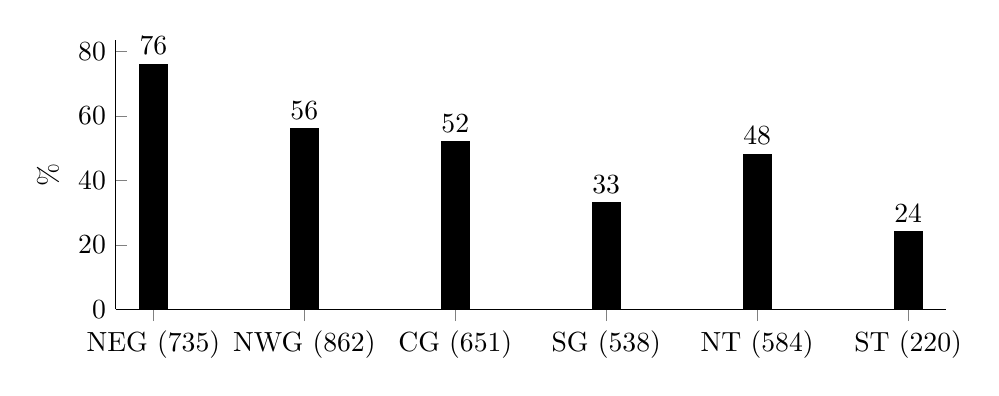
\begin{tikzpicture}
  \begin{axis}
    [ybar,
     axis lines*=left,
     symbolic x coords = {NEG (735),NWG (862),CG (651),SG (538),NT (584),ST (220)},
     xtick=data,
     width=\textwidth,
     height=5cm,
     nodes near coords,
     ylabel = {\%},
     enlarge x limits={0.05},
     ymin=0,
     ylabel near ticks
     ]
    \addplot [fill=black] coordinates {(NEG (735),76) (NWG (862),56) (CG (651),52) (SG (538),33) (NT (584),48) (ST (220),24)};
  \end{axis}
\end{tikzpicture}
\caption{Frequency of clitic doubling in Albanian dialects. The bars display relative frequencies of clitic doubling in each dialect area. The number in brackets next to the abbreviation for the dialect area shows the absolute total number of cases of accusative objects for that specific area.\label{fig7}}
\end{figure}
\il{Albanian}

In general, the frequency pattern in \figref{fig7} corroborates the existence of an increasing frequency of clitic doubling towards the North of the \ili{Albanian} speaking territory \citep[310]{Curtis2012}. This picture would be immaculate if it was not for the high frequency of clitic doubling in \ili{North Tosk} (52\%), which comes as a surprise and does not correspond to the overall areal tendency. A tentative explanation can be found when the same frequency analysis is applied to the areas as defined in \tabref{tab:matoshi:6}, Version B, i.e., considering also the countries the respective dialects are spoken in (cf. \figref{fig8}).

\begin{figure}
\footnotesize
% % % \includegraphics[width=.6\textwidth]{figures/matoshi8.png}
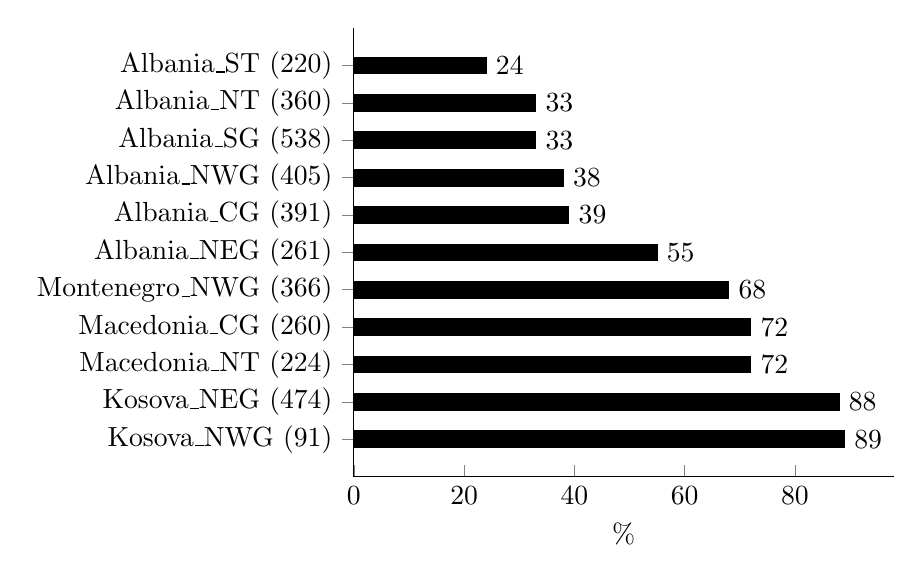
\begin{tikzpicture}
  \begin{axis}
    [xbar,
     axis lines*=left,
     symbolic y coords = {Albania\_ST (220),Albania\_NT (360),Albania\_SG (538),Albania\_NWG (405),Albania\_CG (391),Albania\_NEG (261),Montenegro\_NWG (366),Macedonia\_CG (260),Macedonia\_NT (224),Kosova\_NEG (474),Kosova\_NWG (91)},
     y dir=reverse,
     ytick=data,
     nodes near coords,
     xlabel = {\%},
     xmin=0,
     xlabel near ticks,
     bar width=6pt
     ]
    \addplot [fill=black] coordinates {(24,{Albania\_ST (220)}) (33,{Albania\_NT (360)}) (33,{Albania\_SG (538)}) (38,{Albania\_NWG (405)}) (39,{Albania\_CG (391)}) (55,{Albania\_NEG (261)}) (68,{Montenegro\_NWG (366)}) (72,{Macedonia\_CG (260)}) (72,{Macedonia\_NT (224)}) (88,{Kosova\_NEG (474)}) (89,{Kosova\_NWG (91)})};
  \end{axis}
\end{tikzpicture}
\caption{Frequency of clitic doubling in Albanian dialects considering the countries they are spoken in. The bars display relative frequencies of clitic doubling in each dialect area. The number in brackets next to the abbreviation for the dialect area shows the absolute total number of cases of accusative objects for that specific area. \label{fig8}}
\end{figure}
\il{Albanian}

After including the second classification parameter, i.e. national borders, the areal development of clitic doubling is shown from a completely different perspective: it suggests that the frequency of clitic doubling is to a lesser extent dependent on the dialectal affiliation and/or the geographical area (North vs. South). Of central importance appears to be the division into center and periphery which, more or less, corresponds to the national separation into (a) dialects spoken within the Republic of Albania and (b) dialects spoken in countries of former Yugoslavia (Kosova, Macedonia, Montenegro, Serbia). While \ili{North Albanian} dialects within Albania, especially \ili{Northeast Gheg}, also show a tendency to make more use of clitic doubling, an actual abundance of clitic doubled objects is noticeable only for the dialects spoken outside of Albania. This becomes most obvious when one compares the areas in Albania and Macedonia where \ili{North Tosk} dialects are spoken (Albania: 33\% vs. Macedonia: 72\%). However, it must be emphasized that the rather small amount of data and sparse coverage of the speaking territory requires further studies on the basis of larger amounts of data and focusing especially on the areas along today’s national borders in order to assess the influence of these borders.

Such apparent differences in frequency usually go along with functional differences and require more elaborate analyses, ideally capturing aspects of information structure. However, annotating corpora on the level of information structures has proven to be a cumbersome and error-prone task. Instead, I will draw indirect conclusions on the basis of robust morphological and lexical criteria. According to the introductory remarks in \sectref{sec:matoshi:1}, we arrive at the trivial, yet helpful for the purpose at hand, conclusion that there is a strong tendency for arguments which are given to be also morphologically definite, topicalized and not focused, while newly introduced arguments are usually morphologically indefinite, not topicalized and within the focus domain. What is more, we can state that subjects are better candidates to be topic than objects, which subsequently leads to the conclusion that on a quantitative scale objects commonly tend not to be doubled, which has proven to be correct for most dialects spoken in Albania and especially for \ili{Tosk}, cf. \figref{fig7}. Lastly, I contend that pronouns outrank nouns within the referentiality hierarchy, i.e. indefinite pronouns are rated lower than indefinite nouns (for example: \textit{whom} vs. \textit{a man}) and definite pronouns are rated higher than definite nouns (\textit{him} vs. \textit{the man}).   

This correlation between definiteness and topic acceptability allows for the sketching of clitic doubling frequency patterns along a morpho-lexical definiteness hierarchy, cf. \tabref{tab:matoshi:7}. The classification made here is based on purely morphological and lexical criteria and does not claim to be complete. Thus, for example, the category \enquote{indefinite pronouns} also includes interrogative pronouns. Nevertheless, an additional division of the four classes would lead to an unnecessary complexification and not serve the purpose of the hierarchy, which is to describe general areal tendencies regarding the usage of clitic doubling on a quantitative scale and to compare these findings with the descriptions we find in the current literature on \ili{Albanian} and other Balkan languages.

\begin{table}
\caption{Morpho-lexical definiteness hierarchy.\label{tab:matoshi:7}}
\fittable{\begin{tabular}{lll}
\lsptoprule
1. definite pronouns (prop\_def) & \multirow{4}{*}{\huge$\uparrow$} & \multirow{4}{*}{Increasing frequency of clitic doubling}\\
2. definite nouns (np\_def) & \\
3. indefinite nouns (np\_indef) & \\
4. indefinite pronouns (prop\_indef) & \\        
\lspbottomrule
\end{tabular}}
\end{table}

The underlying assumption is that clitic doubling would increase along this hierarchy, which is confirmed by the results of the corpus analysis for the regions Albania\_NT and Albania\_ST ($\approx$ \ili{Standard Albanian}), cf. \figref{fig9}.

\begin{figure}
\footnotesize
% % \includegraphics[width=0.75\textwidth]{figures/matoshi9.png}
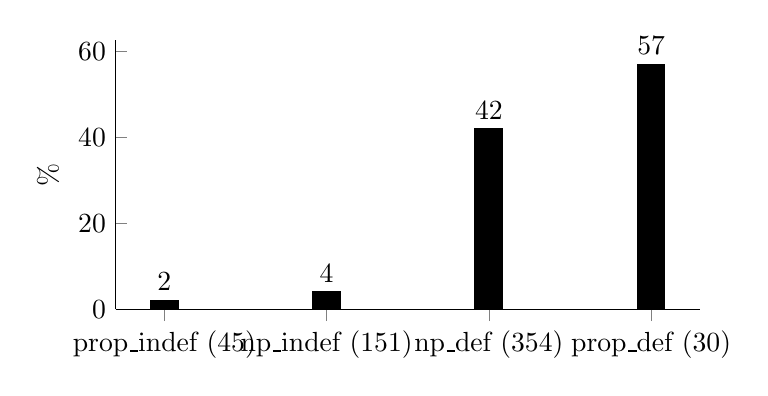
\begin{tikzpicture}
  \begin{axis}
    [ybar,
     axis lines*=left,
     symbolic x coords = {prop\_indef (45),np\_indef (151),np\_def (354),prop\_def (30)},
     xtick=data,
     height=5cm,
     width=9cm,
     nodes near coords,
     ylabel = {\%},
     ymin=0,
     ylabel near ticks
     ]
    \addplot [fill=black] coordinates {(prop\_indef (45),2) (np\_indef (151),4) (np\_def (354),42) (prop\_def (30),57)};
  \end{axis}
\end{tikzpicture}
\caption{Frequency of clitic doubling in the regions Albania\_NT and Albania\_ST along the morpho-lexical definiteness hierarchy. The bars display relative frequencies of clitic doubling. The number in brackets shows the absolute total number of cases of accusative objects.\label{fig9}}
\end{figure}

As the figure shows, clitic doubling mostly occurs in association with definite objects. Despite this strong tendency, definiteness cannot be judged as the decisive factor for clitic doubling, otherwise a higher percentage of doubled definite objects would be expected. \tabref{tab:matoshi:8} displays the usage pattern of clitic doubling for each of the subareas as described in \tabref{tab:matoshi:6}, Version B, along the same morpho-syntactic definiteness hierarchy. 

\begin{sidewaystable}
\caption{Frequency of clitic doubling along a morpho-lexical definiteness hierarchy in Albanian dialects, where $n_{cd}$ is the number of cases with clitic doubling and $n_{ao}$ is the total number of accusative objects. \label{tab:matoshi:8}}
\begin{tabular}{lcrrcrrcrrcrr}
\lsptoprule
Dialect regions &                    & $n_{cd}$ & $n_{ao}$ &                    & $n_{cd}$ & $n_{ao}$ &                    & $n_{cd}$ & $n_{ao}$ &                    & $n_{cd}$ & $n_{ao}$ \\
\midrule
Albania\_CG     & \parbox[t]{2mm}{\multirow{11}{*}{\rotatebox[origin=c]{90}{prop\_indef}}} & 1 (6\%)                  & 16                                 & \parbox[t]{2mm}{\multirow{11}{*}{\rotatebox[origin=c]{90}{np\_indef}}} & 12 (13\%)                & 93                                 & \parbox[t]{2mm}{\multirow{11}{*}{\rotatebox[origin=c]{90}{np\_def}}} & 137 (51\%)               & 269                                & \parbox[t]{2mm}{\multirow{11}{*}{\rotatebox[origin=c]{90}{prop\_def}}} & 4 (31\%)                 & 13                                 \\
Albania\_NEG    &                    & 1 (8\%)                  & 13                                 &                    & 23 (55\%)                & 42                                 &                    & 112 (57\%)               & 197                                &                    & 8 (89\%)                 & 9                                  \\
Albania\_NT     &                    & 0 (0\%)                  & 24                                 &                    & 5 (5\%)                  & 93                                 &                    & 100 (44\%)               & 226                                &                    & 14 (82\%)                & 17                                 \\
Albania\_NWG    &                    & 1 (3\%)                  & 32                                 &                    & 14 (16\%)                & 87                                 &                    & 131 (48\%)               & 275                                &                    & 7 (64\%)                 & 11                                 \\
Albania\_SG     &                    & 0 (0\%)                  & 34                                 &                    & 9 (6\%)                  & 152                                &                    & 150 (47\%)               & 322                                &                    & 20 (67\%)                & 30                                 \\
Albania\_ST     &                    & 1 (5\%)                  & 31                                 &                    & 1 (2\%)                  & 58                                 &                    & 48 (38\%)                & 128                                &                    & 3 (23\%)                 & 13                                 \\
Kosova\_NEG     &                    & 2 (5\%)                  & 38                                 &                    & 85 (90\%)                & 94                                 &                    & 321 (97\%)               & 332                                &                    & 10 (100\%)               & 10                                 \\
Kosova\_NWG     &                    & 0 (0\%)                  & 9                                  &                    & 7 (100\%)                & 7                                  &                    & 69 (99\%)                & 70                                 &                    & 5 (100\%)                & 5                                  \\
Macedonia\_CG   &                    & 0 (0\%)                  & 22                                 &                    & 21 (35\%)                & 60                                 &                    & 161 (93\%)               & 174                                &                    & 4 (100\%)                & 4                                  \\
Macedonia\_NT   &                    & 1 (5\%)                  & 20                                 &                    & 3 (9\%)                  & 33                                 &                    & 142 (92\%)               & 154                                &                    & 15 (88\%)                & 17                                 \\
Montenegro\_NWG &                    & 1 (4\%)                  & 28                                 &                    & 67 (69\%)                & 97                                 &                    & 173 (75\%)               & 230                                &                    & 9 (82\%)                 & 11                                \\
\lspbottomrule
\end{tabular}
\end{sidewaystable}
\il{Albanian}

Of particular interest remain the areas outside the Republic of Albania. The patterns allow for positing grammaticalization along the morpho-syntactic definiteness scale: first, clitic doubling will become almost obligatory with definite pronominal objects, a process that is already in progress for some varieties in North Albania. Then definite nominal objects will follow as the main trigger of clitic doubling while still excluding most indefinite nominals, a stage that has been reached especially in Southwest Macedonia. Subsequently, instances of doubled indefinite nominal objects will become more common, as is the case in Northwest Macedonia. Eventually, the majority of indefinite nominals will undergo clitic doubling in almost any context, a stage that has been reached in Montenegro and, even more so, in Kosova. Novel indefinite pronominal objects, however, remain very resistant to clitic doubling. 

It is important to stress that \tabref{tab:matoshi:8} displays a continuous grammaticalization path and that exceptions from the general tendencies do occur in all of the areas in question. In the following, the \ili{Albanian} speaking territories of Montenegro, Macedonia and Kosova will be subject to a cursory examination from a functional perspective. The leading question will be whether the higher degree of grammaticalization and frequency of clitic doubling in these areas can be viewed as a higher degree of functional transparency.\largerpage

The entire region of Montenegro appears to be most opaque regarding the functional motivation of clitic doubling. On the one hand, the dense occurrence of clitic doubling shows a clear development towards a loss of any restrictions whatsoever, a pattern that comes close to the situation we find in Kosova. This is, however, inconsistent with the relatively high number of exceptions: while most indefinite and definite nominals are doubled, a relatively large number of them are not. See, for instance, example (\ref{example13matoshi}), which presents the beginning of a story: The first object (\textit{i djalë} ‘a son’) is not doubled, which is less surprising as it has the feature matrix [\textminus{}given, \textminus{}definite, \textminus{}topic, +focus] and corresponds to the pattern of \ili{Standard Albanian}. Note, however, that in the subsequent part of the introduction all other instances of an object undergo clitic doubling independent of whether they are [+given/\textminus{}given], [+def/\textminus{}def], [+topic/\textminus{}topic], [+focus/\textminus{}focus].

\ea \label{example13matoshi}
	\langinfo{Northwest Gheg}{Montenegro}{42.44626, 19.4564}\\
	\textit{Â’ kenë i nanë e ka pa’ \uline{i djalë}. Ajo â’ kenë fukara e \uline{e} ka çuo \uline{djalin} rrogtar për me mujë me jetuo. Djali â’ kenë qiros edhe ka tejë tu ‘i zotni rrogtar. ‘I ditë prej ditsh djali â’ ba me do fmi e kanë luoj bashkë. Njari prej asi fmísh e ka pa’ \uline{i kapicë} ën krye. Qirosi i ka lakmuo kapicës edhe prej atyt shkon fill tu nana e vet e i thotë: - Me m\uline{a} ble ‘\uline{i kapicë}! Nana i përgjégj: - T\uline{a} ka pa’ lanë baba ‘\uline{i kapicë}, por po ta gjêj.}
	\glt ‘Once upon a time there was a mother and she $\varnothing$ had \uline{a son}. She was poor and \textsc{cl} sent \uline{her son} as a day laborer so that they would survive. The boy was bald and stayed with a lord as a day laborer. One day the boy gathered with some children and they played together. One of the children \textsc{cl} had \uline{a hat} on his head. The bald boy also wanted such a hat and went from there to his mother and said: \enquote{Buy \textsc{cl} me \uline{a hat}!}. The mother answers him: \enquote{Your father \textsc{cl} left you \uline{a hat}, I will find it for you}.’\il{Northwest Gheg}
\z

Especially in need of explanation are undoubled definite nouns. Later on, in the same story, a magic flute is introduced and doubled when it is mentioned the first time, cf. (\ref{example14matoshi}). The flute plays an important role in the subsequent part of the story (as it empowers the boy to summon a large army whenever he likes) and, therefore, is mentioned several times in the storyline. Nevertheless, in example (\ref{example15matoshi}) when a reference is made to the \enquote{story behind the flute} (\textit{punën e fellit}) the respective object is not doubled.\largerpage

\ea \label{example14matoshi} 
	\langinfo{Northwest Gheg}{Montenegro}{42.44626, 19.4564}\\
	\textit{I ditë prej ditsh bâhet me çobana e j\uline{a} sheh njaj çobanit \uline{fellin} tye i ra. Prap shkon e i thotë nanës: - Nanë, me m\uline{a} ble ‘\uline{i fyell}! Nana i përgjégj: - Qiroso, Qiroso, ma prune punën gusht! T\uline{a} ka pa lanë baba ‘\uline{i dreq fellit}, por ruoju, se ke me ja pa sherrin! Çohet nana, ja gjê e j\uline{a} nep \uline{fellin}.}
	\glt ‘One day he gathers with some shepherds and \textsc{cl} sees \uline{the flute} of a shepherd and him playing with it. Again he goes to his mother and says to her: \enquote{Mother, buy \textsc{cl} me a \uline{flute}}. \enquote{My boy, you really put me in a difficult position! Your father \textsc{cl} left you \uline{a damn flute}, but be careful because it will cause you many more problems!} She gets up, finds it for him and \textsc{cl} gives him \uline{the flute}.’\il{Northwest Gheg}
\ex \label{example15matoshi} 
	\langinfo{Northwest Gheg}{Montenegro}{42.44626, 19.4564}\\
	\textit{- Si â’ kjo punë e ç’ fuqi ke ti qi e ke gjidh kët ushtri? Qirosi, si budallë, i kalzon e i thotë: - Tash me da’ û’, tanë kta periherë i tres mos m’ u duktë ma. Bija e mretit e bvét: - Si muç ti m’ e ba ata? Ky i kuvet krejtsisht \uline{punën e fellit}.}
	\glt ‘\enquote{What's going on and what power do you have that you have this whole army?} The boy, stupid as he was, tells her: \enquote{Now, if I want, I could make the whole army disappear, as if it had never been there}. The king's daughter asks him: \enquote{How can you do that?} He $\varnothing$ tells her in great detail \uline{the story behind the flute}.’\il{Northwest Gheg}
 \z

The status on the level of information structure of the undoubled objects in examples (\ref{example13matoshi}) and (\ref{example15matoshi}) allow us to draw on factors such as focus or givenness in order to explain the absence of the clitic. Such a solution is not satisfactory in as much as it fails to provide a holistic explanation of the usage of clitics in this variety. The scattered instances of clitic omission rather suggest that in the area in question clitic doubling is the default case in association with indefinite nominal and definite nominal and pronominal objects and may be left out facultatively for contrastive or focussing purposes. 

Moving on to the region of West Macedonia, the overall pattern appears to be more transparent. \tabref{tab:matoshi:8} shows that irrespective of the dialectological classification, i.e. \ili{Gheg} vs. \ili{Tosk} variety, in West Macedonia the tendency to almost exclusively double definite objects prevails. This tendency is somewhat stronger in the Southwest area than in the Northwest area where clitic doubling of indefinite objects is more common. In addition, cases with an undoubled definite object are recorded as well. This leads to the intricate question of how to account for these cases which clearly deviate from the overall pattern. Additional factors, alongside definiteness, such as specificity, focus or contrast, have been brought up in the current literature on clitic doubling in \ili{Macedonian}, the main contact language \citep[cf. for example][]{Friedman2008} which shows similar tendencies to double exclusively definite objects. While some cases, such as (\ref{example16matoshi}), clearly suggest contrast, alongside focus, as an important co-factor which prohibits clitic doubling in combination with definite objects, others are harder to account for, such as (\ref{example17matoshi}): the object \textit{një plakë} ‘an old woman’ is doubled despite being [\textminus{}given, \textminus{}definite, \textminus{}topic, +focus]. A possible explanation could be found if the referent is viewed as being [+specific]. Drawing on specificity is also corroborated by example (\ref{example18matoshi}) which is comparable to (\ref{example17matoshi}): the first mentioning of \textit{ni qakë} ‘an old woman’ [\textminus{}given, \textminus{}definite, \textminus{}topic, +focus] is not doubled and, therefore, adheres to the general areal tendency. However, the second instance of the same phrase \textit{ni qakë} ‘an old woman’ undergoes clitic doubling despite having the same features [\textminus{}given, \textminus{}definite, \textminus{}topic, +focus]. One possible explanation would be to view the first instance as [\textminus{}specific], as it does not make any reference to a specific person in the story, and the second as [+specific] since it refers to a specific person in the story. 

\ea \label{example16matoshi} 
	\langinfo{Central Gheg}{Macedonia}{42.03503, 20.9161}\\
	\gll Gje kërkojshe \uline{shatkën}, sot kërkojshe \uline{shatokin}\\
	yesterday want\textsc{.ipf.2sg} duck\textsc{.acc.def} today want.\textsc{ipf.2sg} drake.\textsc{acc.def}\\
	\glt ‘Yesterday you $\varnothing$ asked for \uline{the duck}, today you $\varnothing$ asked for \uline{the drake}.’\\
\ex \label{example17matoshi} 
	\langinfo{North Tosk}{Macedonia}{41.09028, 21.01325}\\
	\textit{oxha ja vuri synë kësaj // po kjo mazalla s’ e deshte // si t’ ja bëjë ?! \uline{e} thiri \uline{një plakë} t’ ia ndreqë punën // plaka tha : unë do ta regulloj që të marë // plaka mori një perusti dhe e vuri tersëne // çupa i thotë : moj plakë / nuku viet ashtu perustija / po ndryshe viet // po nuku di // zbrit e më trego //}
	\glt ‘the Imam had an eye on her [the girl] // but she didn't want anything from him // what should he do now ?! he \textsc{cl} called \uline{an old woman} to settle the matter for him // the old woman said: I'll make sure she takes you // the old woman took a tripod and puts it upside down // the girl says : you there / you don't put a tripod up like this // I don't know // come down and show me //’\il{North Tosk}
\ex \label{example18matoshi} 
	\langinfo{Central Gheg}{Macedonia}{41.23853, 20.64221}\\
	\textit{Hajduti i porosojti : Çitni \uline{ni qakë} t’ lipe vjom devje n’ at mahallë ku u vdir devja , se ai deven e ka therrë ! E qaka, kur t’ dale ne ta boe derën pagës me vjom! Mbasandoj ju shkoni bastojsni ! \uline{E} çesin \uline{ni qakë} . Qaka i merr shpojt me rent.}
	\glt ‘The thief told them, \enquote{$\varnothing$ Send \uline{an old woman} to beg for camel fat in the area where the camel disappeared, because he [the other thief] slaughtered the camel already! And the woman, when she goes out of the house again, let her mark the front door with camel fat! Then you can search the house!} They \textsc{cl} send \uline{an old woman} out. The old woman takes the houses one by one.’
 \z

While the argumentation above seems coherent, one cannot get around the fact that such explanations always bear a certain amount of vagueness and posit a certain degree of arbitrariness and optionality. In any case, drawing on specificity cannot explain the lack of clitic doubling in (\ref{example19matoshi}), as there is no reason why the referent \textit{një çupë} ‘a daughter’, the main figure in the story, should not be regarded as being [+specific]. 

\ea \label{example19matoshi} 
	\langinfo{North Tosk}{Macedonia}{40.8876, 21.31207}\\
	\gll qënka një plak edhe një plakë / kanë edhe një çupë //\\
	be\textsc{.prs.adm.3sg} a old\_woman and a old\_man {} have.\textsc{prs.3pl} also a daughter.\textsc{acc}\\
	\glt ‘once upon a time there was an old woman and an old man / they $\varnothing$ had \uline{also a daughter}’\il{North Tosk}
 \z

It should be emphasized that the entire \ili{Albanian}-speaking territory of Macedonia poses another difficulty, its dialectological heterogeneity. A more fragmented division of the area into a northern, central and southern part would do more justice to the increasing frequency of clitic doubling towards the North where the varieties are actually (transitional to) \ili{Northeast Gheg} and feature a similarly high frequency of clitic doubling as in the \ili{Albanian} varieties of Kosova. It is also Northwest Macedonia where we find a case with a doubled indefinite pronoun \textit{kërkân} ‘no one’, cf. (\ref{example20matoshi}). Note that \citet{Friedman2006} proved the existence of such cases in \ili{Slavic} dialects of Northern Macedonia, as well.

\ea \label{example20matoshi} 
	\langinfo{Northeast Gheg}{Macedonia}{42.16205, 21.61688}\\
	\gll ama kërkân s' un p' e zanë tu vedhë \\
	but no\_one\textsc{.acc} \textsc{neg} can \textsc{prog} \textsc{cl.acc.3sg} catch.\textsc{prs.3pl} \textsc{ger} steal.\textsc{ptcp}\\
	\glt ‘but he couldn't \textsc{cl} catch anyone stealing’\il{Northeast Gheg}
  \z

The varieties in Kosova, both Northeast\il{Northeast Gheg} and \ili{Northwest Gheg}, show a higher degree of homogeneity regarding the usage pattern of clitic doubling which is subject to barely any restrictions whatsoever. While the overall picture is reminiscent of the findings on \ili{Albanian} dialects in the \ili{Montenegrin} area, the usage of clitic doubling is more pervasive and fewer exceptions occur. Most objects without clitic doubling fall under the category of indefinite and interrogative pronouns, and only sporadic instances of undoubled nominals can be found. Example (\ref{example21matoshi}) shows the interrogativ pronoun \textit{kâ} ‘whom’ that is not doubled.

\ea \label{example21matoshi} 
	\langinfo{Northwest Gheg}{Kosova}{42.73953, 20.05389}\\
	\gll Kâ po pret ktu?\\
	whom \textsc{prog} wait.\textsc{prs.2sg} here\\
	\glt ‘\uline{Whom} are you $\varnothing$ awaiting here?’\il{Northwest Gheg}
 \z

Note, however, that in view of example (\ref{example20matoshi}) from North Macedonia, one should actually expect clitic doubling in example (\ref{example21matoshi}). In the analysis, no distinction was made between interrogative pronouns and indefinite pronouns as they mostly do not differ in their form in \ili{Albanian} and share similar features regarding their degree of definiteness and givenness. In this context, it must be stated that example (\ref{example20matoshi}) is marked as it contains a genuine indefinite pronoun in a left-dislocation, in contrast to example (\ref{example21matoshi}) which contains an interrogative pronoun, whose initial position is predefined and not marked in any way. Left-dislocated objects are notoriously associated with topicalization and thus predisposed for clitic doubling \citep[40]{Friedman2008}. In order to draw direct comparisons other examples of left-dislocated indefinite pronouns are required. Unfortunately, these cases are very rare in the corpus used so far for quantitative comparisons. Thus, additional material from the folkloristic literature from the region of Drenica in central Kosova (hereafter called Drenica corpus) was searched manually. The search unveiled other cases of left-dislocated indefinite pronouns; clitic doubling occurred in two of them, cf. (\ref{example22matoshi}) and (\ref{example23matoshi}). Nevertheless, not all instances of left-dislocation indefinite pronouns are doubled, cf. (\ref{example24matoshi}).  

\ea \label{example22matoshi} 
	\langinfo{Northeast Gheg}{Kosova}{42.52, 20.85527 (Drenica corpus)}\\
	\gll Pos teje \uline{qeterkan} për nafakë nuk \uline{e} due.\\
	except\_for you no\_one.\textsc{acc} for fate \textsc{neg} \textsc{cl.acc.3sg} want\textsc{.prs.1sg}\\
	\glt ‘\uline{No one} else I \textsc{cl} want as my husband except for you.’\il{Northeast Gheg}
\ex \label{example23matoshi} 
	\langinfo{Northeast Gheg}{Kosova}{42.52, 20.85527 (Drenica corpus)}\\
	\gll Une \uline{qetërkân} për nafakë nuk \uline{e} due vetëm ktâ \\
	I no\_one.\textsc{acc} for fate \textsc{neg} \textsc{cl.acc.3sg} want.\textsc{prs.1sg} only him\\
	\glt ‘\uline{No one} else I \textsc{cl} want as my husband, only him.’\il{Northeast Gheg}
\ex \label{example24matoshi} 
	\langinfo{Northwest Gheg}{Kosova}{42.73953, 20.05389}\\
	\gll \uline{Tjetër} \uline{gjâ} s’ folën motrat.\\
	other thing\textsc{.acc} \textsc{neg} speak.\textsc{aor.3pl} sister.\textsc{nom.pl.def}\\
	\glt ‘\uline{something else} the sisters didn’t $\varnothing$ speak’\il{Northwest Gheg}
 \z

The fact that all three cases (\ref{example20matoshi}), (\ref{example22matoshi}) and (\ref{example23matoshi}) with clitic doubled indefinite pronouns are [+human] deserves attention and raises the question whether the additional semantic factor [+human\slash\textminus{}human] must be considered. Against this background the following excerpts from newspaper articles extracted from the \ili{Albanian} National Corpus\footnote{\url{http://web-corpora.net/AlbanianCorpus/search/}}  may be classified as evidence for an ongoing or already completed grammaticalization process towards an obligatory clitic doubling of indefinite (including interrogative) pronouns which have the semantic feature [+human]:

\ea \label{example25matoshi} 
	\normalfont{{Kosova sot}}\footnote{\url{https://www.kosova-sot.info/lajme/19663/ndihmohen-femijet-e-drenices-ja-ke-e-falenderon-e-ke-e-shan-milaim-zeka/}}\\
	\gll Ja kë e falënderon e kë e shan M. Z.\\
	here whom \textsc{cl.acc.3sg} thank.\textsc{prs.3sg} and whom \textsc{cl.acc.3sg} scold.\textsc{prs.3sg} M. Z.\\	
	\glt ‘One can tell \uline{whom} M. Z. \textsc{cl} thanks and \uline{whom} he \textsc{cl} scolds.’
 \z
 
The sentences above appeared in newspapers from Kosova. Newspapers from Kosova contain many cases of clitic doubling with the interrogative pronouns \textit{kë} `whom'. This is remarkable in the sense that the same standard variety is used as the official language in Kosova, Albania and in the \ili{Albanian} communities of Macedonia. The fact that the authors of the articles were not aware of this redundant use of clitic doubling may serve as an indicator for how far the grammaticalization process has gone in these varieties. Nevertheless, further studies with the aid of larger corpora and/or experiments are required to furnish proof.  
 
The last desideratum that remains is to explain the cases with undoubled indefinite and definite nominals in the \ili{Albanian} varieties of Kosova, which do not match the overall pattern at all. Their scattered occurrence allows for several different tentative explanations, all of them implying that clitic doubling serves an expressive function, leaving its omission in some cases at the discretion of the speaker. A similar conclusion by drawing on optionality was also made for the region of Montenegro to explain the rather arbitrary cases of clitic omission. One such explanation can be found in \citet[192--193]{Buchholz1977}, who contends that the omission of clitic doubling in combination with non-novel definite objects emphasizes a change in the situation. Indeed, some examples with undoubled definite objects describe a turning point, such as (\ref{example26matoshi}), where the word order V O S is also marked. Example (\ref{example27matoshi}) is \enquote{marked} as well, in as much as the respective clause without clitic doubling is embedded in a chain of successive short clauses and therefore conveys a certain degree of dynamicity. Other cases, such as (\ref{example28matoshi}), speak in favor of viewing the associated object not as definite, despite its definite affix, but as a component of an incorporation into the verb, since the meaning of the noun-verb construction is not compositional. Example (\ref{example29matoshi}), on the other hand, remains opaque since the object is not only [+given,+topic,+definite,\textminus{}focus] it is also left-dislocated and therefore expected to undergo clitic doubling. 
 
\ea \label{example26matoshi} 
	\langinfo{Northeast Gheg}{Drenica corpus}{}\\
	\gll Kap \uline{shtagën} baba e shko tu begu\\
	grab.\textsc{prs.3sg} stick\textsc{.acc.def} father.\textsc{nom.def} and go.\textsc{prs.3sg} to bey\textsc{.nom.def}\\
	\glt ‘The father $\varnothing$ takes the \uline{stick} and goes to the bey.’\il{Northeast Gheg}
\ex \label{example27matoshi} 
	\langinfo{Northeast Gheg}{Kosova}{42.38441, 20.4285}\\
	\gll Çohet / e kish pas marr etja // niset për shpi // lyp \uline{kofen} \uline{e} \uline{bunarit} me pi uj // kofa kërkun\\
	get\_up\textsc{.prs.pass.3sg} {} \textsc{cl.acc.3sg} have\textsc{.prs.3sg} have\textsc{.ptcp} take\textsc{.ptcp} thurst.\textsc{nom.def} {} set.off\textsc{.prs.pass.3sg} for home {} look\_for.\textsc{prs.3sg} bucket.\textsc{acc.def} \textsc{art} well.\textsc{gen.def} \textsc{inf} drink\textsc{.ptcp} water {} bucket.\textsc{nom.def} nowhere\\
	\glt ‘he stands up / he was thirsty // he heads for home // he $\varnothing$ seeks the \uline{well bucket} to drink water // the bucket was nowhere’\il{Northeast Gheg}
\ex \label{example28matoshi} 
	\langinfo{Northeast Gheg}{Kosova}{42.38441, 20.4285}\\
	\gll Muer \uline{dyjênë} n’ sy Baba Hasani për m’ u largue pej shpije.\\
	take\textsc{.aor.3sg} world\textsc{.acc.def} in eye.\textsc{acc} Baba Hasan \textsc{supin} \textsc{inf} \textsc{pass} leave.\textsc{ptcp} from house\textsc{.abl}\\
	\glt ‘Baba Hasan set off to leave the house.’ (Lit. ‘Baba Hasan $\varnothing$ took \uline{the world} in his eye to leave the house’)\il{Northeast Gheg}\\	
\ex \label{example29matoshi} 
	\langinfo{Northwest Gheg}{Kosova}{42.73953, 20.05389}\\
	\gll Mreti u kallxoi : – \uline{Qeso} \uline{héshë} veç grueja m’ goditke!\\
	king.\textsc{nom.def} \textsc{cl.dat.3pl} tell\textsc{.aor.3sg} {} {} this\_kind\_of food\textsc{.abl} only wife\textsc{.nom.def} \textsc{cl.dat.1sg} make.\textsc{ipf.3sg}\\
	\glt ‘The king told them: \enquote{\uline{This kind of food} only my wife $\varnothing$ made for me}.’\il{Northwest Gheg}
 \z

\section{Concluding remarks}

Although peripheral \ili{Albanian} dialects outside the Republic of Albania feature a higher frequency of clitic doubling than most \ili{Albanian} dialects spoken in the Republic of Albania, the relatively high number of opaque usage cases does not allow us to view the redundant use of clitic doubling as evidence of a higher degree of functional transparency and, therefore, as a language change for the better. In case of \ili{Standard Albanian}, most instances of clitic doubling in main clauses allowed for an explanation by defining whether the respective object was [+focus, \textminus{}topic] or not. While notions, such as \textit{topic} or \textit{focus}, prove to be intricate at first glance, once detected they can be applied to explain almost any instance of clitic doubling in \ili{Standard Albanian}.
% Even those cases which were deemed exceptions, cf. (\ref{example9matoshi}) and (\ref{example10matoshi}), were largely compatible with the overall systematicity.
In the case of the dialects outside Albania, the data allowed for the sketching of an interim and coarse usage pattern along a morpho-lexical definiteness hierarchy which seems neat \textit{prima facie} and suggests more easily detectable factors, to wit \textit{definiteness}. 

However, it is all the more difficult to explain cases which do not adhere to this usage pattern. In particular need of explanation are cases with undoubled definite objects. In contrast to \ili{Standard Albanian}, one must avail oneself of additional factors, such as \textit{contrast}, cf. (\ref{example16matoshi}), \textit{specificity}, cf. (\ref{example17matoshi}), (\ref{example18matoshi}), or even \textit{animacy}, cf. (\ref{example22matoshi}), (\ref{example23matoshi}), to explain the exceptional cases. What is even more important, the explanations offered in the work at hand are tentative and far from sufficient and do not offer a holistic description. The rather scattered and unsystematic cases of clitic omission in combination with indefinite nominals and definite nominals, especially in \ili{Albanian} varieties spoken in Montenegro and Kosova, and the difficulties of pinning down clear factors suggest a certain degree of optionality, which is not given in \ili{Standard Albanian} and presumably in the majority of varieties spoken in the Republic of Albania. Thus, from a descriptive point of view, with the claim of finding regularities with a great amount of certainty, optionality can be regarded as an indicator of a higher degree of functional opaqueness. 

\section*{Abbreviations}
\begin{multicols}{2}
\begin{tabbing}
SUPIN\hspace{1ex} \= \ili{Northeast Gheg}\kill
1               \> first person\\
2               \> second person\\
3               \> third person\\
\textsc{abl}    \> ablative\\
\textsc{acc}    \> accusative\\
\textsc{aor}    \> aorist\\
\textsc{art}    \> linking article\\
CG              \> \ili{Central Gheg}\\ 
\textsc{cl}     \> clitic\\
CT              \> \ili{Cham Tosk}\\
\textsc{dat}    \> dative\\
\textsc{def}    \> definite\\
\textsc{gen}    \> genitive\\
\textsc{ger}    \> gerund\\
\textsc{imp}    \> imperative\\
\textsc{inf}    \> infinitive\\
\textsc{ipf}    \> imperfect\\
\textsc{neg}    \> negation, negative\\
NEG             \> \ili{Northeast Gheg}\\
\textsc{nom}    \> nominative\\
NT              \> \ili{North Tosk}\\
NWG             \> \ili{Northwest Gheg}\\
\textsc{pass}   \> passive\\
\textsc{pl}     \> plural\\
\textsc{prog}   \> progressive\\
\textsc{prs}    \> present\\
\textsc{ptcp}   \> participle\\
\textsc{sg}     \> singular\\
SG              \> \ili{South Gheg}\\
ST              \> Lab/South Tosk\il{South Tosk}\\
\textsc{supin}  \> supin.
\end{tabbing}
\end{multicols} 
 
{\sloppy\printbibliography[heading=subbibliography,notkeyword=this]}

\end{document}

% Anmerkungen:
%
% Table fig10 ist eine Interpretation von mir, weil die Originaltabelle viel zu groß ist.
